%Przykładowy plik ułatwiający złożenie projektu dyplomowego inżynierskiego.
%UWAGA: Generowany napis na stronie tytułowej o treści PROJEKT DYPLOMOWY INŻYNIERSKI został zaproponowany przeze mnie i nie jest, póki co, potwierdzony przez władze wydziału. Przed ostatecznym oddaniem tak złożonej pracy należy upewnić się jaka powinna być treść tego napisu. W momencie gdy uzyskam informację na temat treści tego napisu, dokonam niezbędnych zmian w źródłach.

\documentclass[eng,printmode]{mgr}
%opcje klasy dokumentu mgr.cls zostały opisane w dołączonej instrukcji

%poniżej deklaracje użycia pakietów, usunąć to co jest niepotrzebne
\usepackage{polski} %przydatne podczas składania dokumentów w j. polskim
%\usepackage[polish]{babel}%alternatywnie do pakietu polski, wybrać jeden z nich
\usepackage[utf8]{inputenc} %kodowanie znakĂłw, zaleĹĽne od systemu
\usepackage[T1]{fontenc} %poprawne składanie polskich czcionek

%pakiety do grafiki
\usepackage{graphicx}
%\usepackage{subfigure}
\usepackage{psfrag}

%pakiety dodające dużo dodatkowych poleceń matematycznych
\usepackage{amsmath}
\usepackage{amsfonts}

%pakiety wspomagające i poprawiające składanie tabel
%\usepackage{supertabular}
\usepackage{array}
\usepackage{tabularx}
\usepackage{hhline}

%pakiet wypisujący na marginesie etykiety równań i rysunków zdefiniowanych przez \label{}, chcąc wygenerować finalną wersję dokumentu wystarczy usunąć poniższą linię
%\usepackage{showlabels}

%definicje własnych poleceń
\newcommand{\R}{I\!\!R} %symbol liczb rzeczywistych, działa tylko w trybie matematycznym
\newtheorem{theorem}{Twierdzenie}[section] %nowe otoczenie do składania twierdzeń

%dane do złożenia strony tytułowej
\title{Detekcja aktywności mówcy w systemach automatycznego rozpoznawania mowy}
\engtitle{Voice activity detection in automatic speech recognition systems}
\author{Paulina Szczerbak}
\supervisor{Prof. dr hab. inż. Ryszard Makowski}
%\guardian{dr hab. inż. Imię Nazwisko Prof. PWr, I-6} %nie używać jeśli opiekun jest tą samą osobą co prowadzący pracę

%\date{2008} %standardowo u dołu strony tytułowej umieszczany jest bieżący rok, to polecenie pozwala wstawić dowolny rok

%poniżej jest lista kierunków i specjalności na wydziale elektroniki, należy wybrać właściwe lub dopisać jeśli nie ma odpowiednich
\field{Automatyka i Robotyka (AIR)}
\specialisation{Technologie informacyjne w systemach automatyki (ART)}

%tutaj zaczyna się właściwa treść dokumentu
\begin{document}
\bibliographystyle{plabbrv} %tylko gdy uĹĽywamy BibTeXa, ustawia polski styl bibliografii

\maketitle %polecenie generujące stronę tytułową
%\dedication{6cm}{Dla mamy i taty heheheheheh xD \texttt{$\backslash$dedykacja}}

\tableofcontents %spis treści

%poniżej znajduje się przykładowa treść dalszej części dokumentu, zainteresowanych zachęcam do rozszyfrowania frazy "Lorem ipsum" :)
\chapter{Wstęp}
Celem niniejszej pracy jest zaprezentowanie wybranych metod detekcji aktywności mówcy (VAD) w systemach automatycznego rozpoznawania mowy w oparciu o napisany program w języku C++. Kolejnym etapem jest porównanie zaimplementowanych metod pod względem dokładności detekcji w separowanych wyrazach oraz w dłuższych ciągach słów.

Rozdział 2. opisuje w uproszczony sposób proces wytwarzania mowy przez człowieka. Prezentuje, w jaki sposób działa aparat mowy oraz z jakich narządów się składa. Wyjaśnione zostaje zagadnienie fonemów oraz ich wykorzystanie w polskim alfabecie. Na koniec pokazany jest matematyczny model jaki można stworzyć wzorując się na naturalnym systemie generowania mowy.

Rozdział 3. zawiera wyjaśnienie na temat detekcji aktywności mówcy - czym jest oraz gdzie jest wykorzystywana. W tym rodziale opisane są również wybrane algorytmy, które zostały zestawione w dalszej części pracy. Przedstawiona jest zasada ich działania oraz pokrótce wyjaśniona kwestia implementacyjna każdego z nich.
 
Rozdział 4. prezentuje wyniki działania wybranych algorytmów dla separowanych słów. Pokazane są różnice w detekcji oraz ocena każdego z algorytmów.

Rozdział 5. zawiera  wyniki detekcji dla całych ciągów słów oraz porównanie w działaniu wybranych algorytmów i ich ocenę.

\chapter{Generowanie sygnału mowy}
 \section{Mowa w życiu człowieka}
 
 Mowa w życiu większości ludzi stanowi podstawę komunikacji interpersonalnej. Jest sygnałem akustycznym, czyli rozważany jest zakres częstotliwości słyszanych przez człowieka, to jest od 20Hz do 16kHz. Zatem mowa to nic innego jak system artykułowanych dźwięków, które układają się zgodnie z konwencją wybranego języka. Pełni ona funkcję nie tylko komunikacyjną (przekazywanie informacji drugiej osobie o tym, co doświadczyliśmy, czy czego się dowiedzieliśmy), ale również ekspresyjną (można w niej zawrzeć informacje o emocjach nadawcy) oraz regulacyjną (wydawanie i przyjmowanie dyspozycji). 
 
 
 \section{Biologiczny proces generowania mowy}
 Wszelkie metody przetwarzania sygnału mowy muszą bazować na strukturze sygnału, a ta jest niewątpliwie uzależniona od sposobu, w jaki jest on wytwarzany. Niegdyś generowanie sygnałów mowy było domeną jedynie organizmu człowieka, czyli systemu naturalnego. W celu stworzenia systemu, który w jakiś sposób operuje na sygnałach mowy, czyli np. syntezatora mowy, systemu generującego sygnały mowopodobne, systemu automatycznego rozpoznawania mowy czy detekcji aktywności mówcy, należy mieć przynajmniej podstawową wiedzę na temat systemu naturalnego - tego, w jaki sposób działa aparat mowy człowieka.
 
 Wytwarzanie mowy przez człowieka jest procesem niezwykle skomplikowanym, który ma swój początek w mózgu, gdzie następuje konstrukcja wypowiedzi. Później następuje sformułowanie fonetyki i artykulacja poprzez aparat mowy. Ponadto, w procesie generowania mowy można wyróżnić cztery pomniejsze etapy:
	 
	 - proces psychologiczny - wymyślenie i skonstruowanie wypowiedzi,
	 
	 - proces neurologiczny - pobudzenie przez układ nerwowy mięśni, które biorą udział w wytwarzaniu mowy,
	 
	 - proces fizjologiczny - proces kształtowania dźwięków mowy ludzkiej,
	 
	 - proces aerodynamiczny - drgania i przepływ powietrza przez aparat mowy. 
  
  Pierwszym narządem wchodzącym w skład traktu głosowego człowieka są płuca - dostarczają one powietrze do procesu artykulacji, są źródłem zmian ciśnienia akustycznego. Organ mowy człowieka jest napędzany przez wydychane powietrze. Powietrze to, jest prowadzone przez oskrzela i tchawicę do krtani, a drgające w niej struny głosowe modyfikują ciśnienie i wytwarzają dźwięczne fragmenty mowy.  Następnie, dzięki wnękom rezonansowym, tworzonym przez język, podniebienie, zęby oraz wargi, dźwięk ten jest modulowany. Niezwykle ważną rolę przy formowaniu tych wnęk, odgrywają ruchy żuchwy i policzków. Podczas generowania głosek nosowych zamknięta jama ustna spełnia rolę bocznika akustycznego, a dzięki odpowiedniemu ustawieniu języczka podniebienia miękkiego, fala dźwiękowa jest emitowana przez jamę nosową i nozdrza. Struktura traktu głosowego jest przedstawiona schematycznie na rysunku 2.1.

\begin{figure}
	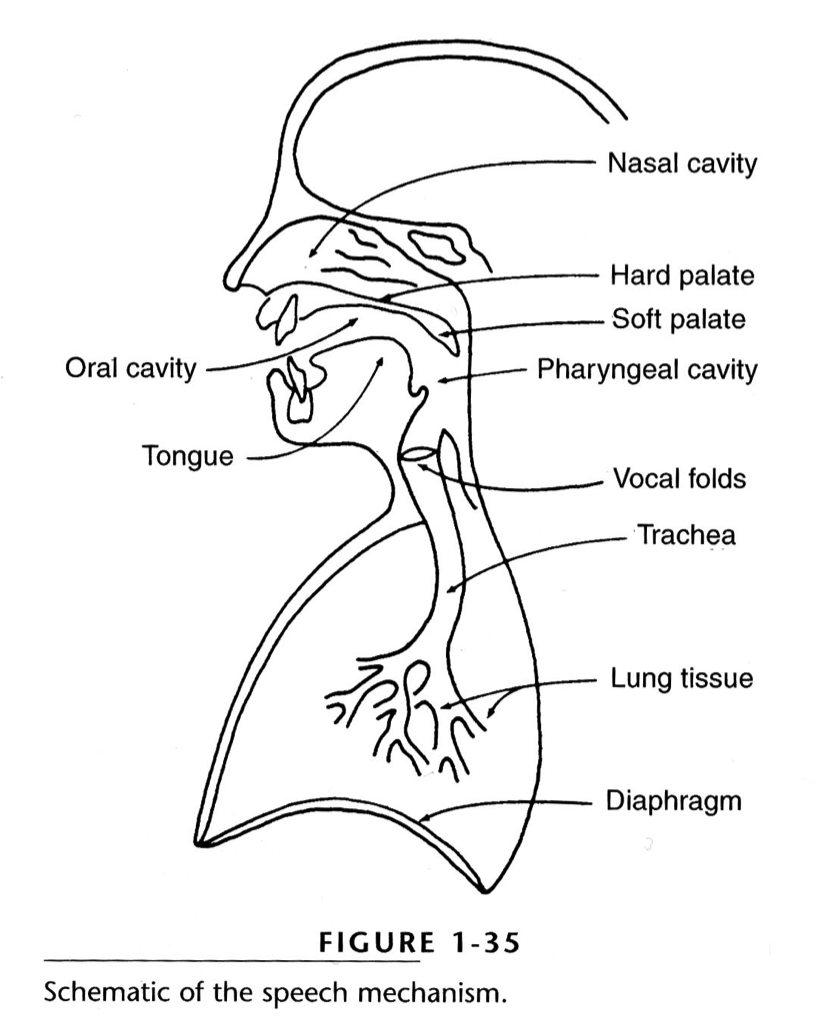
\includegraphics[scale=0.45]{speechmech.png}
	\caption{Aparat mowy człowieka}
\end{figure}

 Ponadto, sterowanie całym systemem generowania mowy jest bardzo złożone i w dużej mierze opiera się na licznych sprzężeniach zwrotnych. Główną rolę odgrywa tutaj sprzężenie zwrotne, które poddaje jakość wydawanych dźwięków bezpośredniej ocenie poprzez analizator słuchowy. Dzięki temu proces artykulacji jest odpowiednio sterowany. Istotę tego sprzężenia zwrotnego potwierdzają trudności z mową wśród ludzi głuchych oraz ludzi słyszących, którzy tymczasowo przebywają w trudnych warunkach środowiskowych, które uniemożliwiają słyszenie własnego głosu.
 
 SCHEMAT Z PDFA STR 23 SPRZERZENIE ZWROTNE  
  
 \section{Jednostki fonetyczne}
 W celu przeprowadzania badań nad sygnałem mowy, należy wprowadzić jednostkę, która ułatwi wykonywanie operacji na całych słowach. Należy tutaj zaznaczyć, że słowo to dźwiękowy odpowiednik wyrazu, a wyraz to zapis słowa. Każde słowo zawiera w sobie przynajmniej jedną sylabę, każdą sylabę można również podzielić na mniejsze stany. W związku z tym, że każdy wyraz zawiera w sobie ciąg liter, to najczęściej wyróżnianymi elementami słowa są fonemy, zwane również głoskami. W większości przypadków na każdy fonem przypada odpowiadająca mu litera, ale są fonemy, które takiego odpowiednika nie posiadają. Istotne jest rownież, że każda litera może mieć różną reprezentację akustyczną w zależnośći od sąsiadujących z nią fonemów. Listę fonemów języka polskiego przedstawiono w tabeli 2.3.1.
 
 TABELA Z FONEMAMI MOWY POLSKIEJ
 
 \section{Matematyczny model procesu generowania mowy}
 
 

\chapter{Wybrane metody detekcji aktywności mówcy}
 \section{Czym jest detekcja aktywności mówcy oraz gdzie się ją wykorzystuje}
 + schemat jak w ksiazce RM, w ktorym miejscu jest vad w systemie ARM
 
 Detekcja aktywności mówcy (Voice Activity Detection - VAD) jest powszechnie stosowana w systemach automatycznego rozpoznawania mowy. Podczas rejestrowania wypowiedzi do późniejszego przetwarzania jej przez system ARM, zostaje zarejestrowana cała wypowiedź mówcy, włącznie z częścią, która nie zawiera mowy. Jeżeli we fragmencie jest zawarty sygnał mowy, mówimy, że mówca jest aktywny. Aktywnością mówcy nazywa się emitowny przez niego dźwięk.  Zawartość semantyczna wypowiedzi jest zawarta w głównej mierze we fragmentach, kiedy mówca jest aktywny. Analizowanie całego  zarejestrowanego sygnału mowy, bez wykorzystania systemu VAD, jest oczywiście możliwe, aczkolwiek niepotrzebnie zwiększa czas obliczeń oraz istnieje prawdopodobieństwo, że fragment, gdy mówca nie jest aktywny, zostanie błędnie zaklasyfikowany jako jakiś konkretny fonem - zatem w dużej mierze może popsuć jakość rozpoznania. Detekcja aktywności mówcy w ogólnym przypadku zakłada, że sygnał może występować w dwóch stanach: tylko szum (brak sygnału mowy), szum + sygnał mowy. Korzystając z zagadnienia hipotez ze statystyki, możemy pierwszy stan oznaczyć jako hipotezę $H_{0}$, a drugi jako $H_{1}$, dzięki czemu możemy przedstawić to w następujący sposób:
 \begin{equation}
  \begin{array}{c}
	  H_{0}: f(n)=x(n)\\
	  H_{1}: f(n)=v(n)+x(n)
  \end{array} 	 
 \end{equation}
  Przy takim rozumowaniu konieczne jest określenie statystyki $S(n)$ sygnału, dzięki czemu możliwe będzie dokonywanie detekcji, a w dalszej kolejności zastosowanie kryterium decyzyjnego. Kryterium decyzyjne zwykle polega na porównaniu wartości $S(n)$ z progiem detekcji, który w mniej skomplikowanych algorytmach przyjmuje stałą wartość. Natomiast w tych bardziej złożonych, może występować np. jako funkcja czasu. Wartość stałej wartości progu jest ustalana w wyniku teoretycznych rozważań lub empirycznie. Zatem detekcja $\gamma(n)$, w ogólnej postaci, będzie prezentować się następująco:
   \begin{equation}
   \begin{array}{c}
	   S(n)\geq\gamma(n)\to H_{1}\\
	   S(n)<\gamma(n)\to H_{0}
   \end{array} 	 
   \end{equation}
 
	MIARY JAKOSCI DETEKCJI DODATEK D 
 

 \section{Algorytm bazujący na energii pojedynczej ramki}
 \section{Algorytm bazujący na obwiedni sygnału}
 \section{Algorytm SFF (Single Frequency Filtering)}
 tłumaczenie artykułu:
 
 Podstawowe informacje w podejściu Single Frequency Filtering
 
 Sygnał mowy ma zależności zarówno z czasem, jak i z częstotliwością. Skutkuje to tym, że SNR (Signal to Noise Ratio) jest funkcją w dziedzinie czasu oraz w dziedzinie częstotliwości. Dla idealnego szumu o danej całkowitej mocy, moc jest podzielona równo dla każdej częstotliwości, podczas gdy dla sygnału moc jest rozdzielona nierównomiernie dla częstotliwości. Zatem, $S^2(f)/N^2(f)$ jest wyższe dla niektórych częstotliwości i niższe dla innych, gdzie S(f) i N(f) są amplitudami sygnału i szumu jako funkcja w dziedzinie częstotliwości. To daje dużo wyższe wartości dla średniej wartości  $S^2(f)/N^2(f)$ powyżej zakresu częstotliwości w porównaniu ze stosunkiem całkowitej mocy sygnału do całkowitej mocy szumu powyżej całkowitego zakresu częstotliwości. 
 
 Przyjmijmy wzory (1), (2), (3) z artykułu, gdzie (fi - fi+1)
 jest (i+1)-tą przerwą spośród L nienachodzących na siebie pasm częstotliwościowych oraz i=0,1,...,L-1. Obowiązuje następująca nierówność:
 
 alfa >= beta >= gamma (4)
 
 S(f) i N(f) są obliczane dla zdegradowanego wyrażenia mowy i dla szumu używając 512-punktowej DFT dla segmentów zokienkowanych oknem Hanna o rozmiarze 20msec dla KAŻDEGO PRZESUNIĘCIA PRÓBKI używając L=16. W Tabeli I (artykuł) przedstawiono średnie wartości alfa, beta, gamma obliczone dla całego wyrażenia. Oczywiste jest, że średine alfa >= średnie beta >= średnie gamma dla różnych typów szumu. W przypadku dla szumu białego wartości sr alfa, sr beta, sr gamma są niższe niż wartości dla niestacjonarnych szumów(np volvo i karabin maszynowy). W przypadku dla szumów niestacjonarnych dolna granica jest niska dla niektórych częstotliwości, co sprawia, że mianownik N(f) jest mały. Z małymi wartościami w mianowniku, współczynniki alfa, beta gamma są relatywnie wyższe, jak zaobserwowano w Tabeli I w srednich wartosciach alfa, beat, gamma dla szumu volvo i karabinu maszynowego. Warto również zauważyć, że dla szumów rozłożonych nierównomiernie, taich jak karabin maszynowy, f16 i volvo, wartości sr alfa i sr beta są dużo wyższe niż dla większości szumów rozłożonych równomiernie, taich jak szum biały, różowy i buccaneer2, podczas gdy odpowiadające im wartości sr gamma są niskie we wszystkich przypadkach. Ma to związek z obszarami zawierającymi wysoki S(f)/N(f) (SNR) w dziedzinie czasu i dziedzinie częstotliwości dla szumów rozłożonych nierównomiernie.
 
 Moc sygnału i szumu jako funkcja w dziedzinie częstotliwości może zostać obliczona wykorzystując  blokowe przetwarzanie jak w DFT lub poprzez filtrowanie przez SFF, jak opisano w następnej skcji. Tabela II pokazuje, że nierówność (4) obowiązuje również w podejściu SFF. Oczekuje się, że zarówno podeście oparte o DFT, jak i SFF dadzą podobne rezultaty. Podejście SFF zostało tutaj wykorzystane, ponieważ dzięki niemu mozna uniknąć niektórych skutków spowodowanych blokowym przetwarzaniem. Również obliczenia dla SFF są szybsze w porównaniu z obliczeniami w DFT w każdej chwili próbkowania.
 
 
 Proponowany algorytm VAD 
 
 A. Obwiednia sygnału mowy w każdej częstotliwości
 
 Sygnał mowy w zdyskretyzowanej dziedzinie czasu s(n) jest różnicowany i zróżnicowany sygnał jest rozumiany jako x(n) = s(n) -s(n-1). Częstotliwość próbkowania to fs. Sygnał x(n) jest przemnażany przez zespolona sinusoidę o danej znormalizowanej częstotliwości śr omega k. Wynikowa operacja w dziedzinie czasu jest dana jako: 
 
 $xk(n) = x(n)e^(j śromegak n)$, gdzie 
 
 $śr omega k = (2pi*śr_fk)/fs.$
 
 Kiedy pomnożymy x(n) przez $e^(j*śr_omega_k*n)$, wynikowe widmo xk(n) będzie przesuniętym widmem x(n). Czyli,
 
$ Xk(omega) = X(omega - śr_omega_k)$,
 gdzie Xk(omega) i X(omega) to odpowiednio widma xk(n) i x(n).
 
 Sygnał xk(n) jest przepuszczany przez jednobiegunowy filtr, którego transmitancja jest dana jako:
 
 $H(z) = 1/(1+rz^(-1)).$
 
 Jednobiegunowy filtr ma biegun na osi liczb rzeczywistych w odległości r od początku układu współrzędnych. Lokalizacja pierwiastka jest w z = -r na płaszczyśnie liczb zespolonych , co odpowiada połowie częstotliwości próbkowania, np fs/2. Wyjście filtra yk(n) jest dane jako:
 
 yk(n) = -r *yk(n-1)+xk(n)
 
 Obwiednia sygnału yk(n) jest dana jako:
 
 $ek(n) = sqrt(ykr^2(n) + yki^2(n))$ (10) , 
 
   gdzie ykr(n) i yki(n) są odpowiednio częścią rzeczywista i urojoną yk(n).
 
 Kiedy filtrowanie xk(n) będzie zrobione dla fs/2, powyższa obwiednia ek(n) będzie odpowiadać obwiedni sygnału xk(n) przefiltrowanego w pożądanej częstotliwości 
 
 $fk = fs/2 - śr_fk.$
 
 
 Powyższa metoda estymowania obwiedni składowej dla częstotliwości fk jest określana jako podejście single frequency filtering (SFF). Wybór filtru z biegunem w z=-r do estymacji obwiedni przefiltrownego sygnału wydaje się być bardziej odpowiedni, jako że obwiednie są obliczane w możliwie najwyższych częstotliwościach (fs/2). Ponadto, wybór filtru w stałej częstotliwości dla jakiejkolwiek pożądaniej częstotliwości fk zapobiega efektu przeskalowania w związku z różnymi wzmocnieniami filtrów w różnych częstotliwościach. Jeżeli biegun jest wybrany na kole jednostkowym, np z=r=-1, może to skutkować niestabilnością wyjścia filtru. Stabilność filtru jest zapewniona dzięki pchnięciu bieguna nieco bardziej wewnątrz koła jednostkowego. Z tego powodu r zostało dobrane jako 0.99.
 
 W tym badaniu obwiednia została obliczona dla każdych 20Hz w przedziale od 300Hz do 3000Hz jako funkcja w dziedzinie czasu. Wybrany został przedział częstotliwości 300-4000Hz, ponieważ pokrywa przydatne widmowe pasma mowy. Zatem mamy obwiednie dla 185 częstotliwości jako funkcja w dziedzinie czasu. Zasadniczo obwiednia może zostać obliczona dla każdej pożądanej częstotliwości.
 
 
 B. Składowe ważone obwiedni sygnału mowy
 
 Kiedy sygnał mowy ma bardzo duży zakres dynamiczny w dziedzinie częstotliwości, sygnał może mieć wysoką wartość mocy w niektórych częstotliwościach w każdej chwili czasowej. W tych częstotliwościach SNR będzie miał większą wartość, jako, że moc szumu będzie prawdopodobnie mniejsza w związku z większym rozkładem jednostajnym mocy. Nawet dla szumów z nierównomiernym rozkładem mocy, niższe korelacje próbek szumu skutkują w niższym dynamicznym zakresie w rozpiętości mocy szumu przez częstotliwość, w porównaniu z sygnałem mowy. Zauważmy, że widmowy zakres dynamiczny daje przejaw korelacji próbek w dziedzinie czasu. 
 
 Moc szumu tworzy funkcję podłogi dla obwiedni dla każdej częstotliwości i poziom podłogi zależy od rozkładu mocy szumu wobec częstotliwości. Podłoga jest bardziej jednorodna wobec czasu, jeżeli szum jest niemalże stacjonarny.Nawet jeżeli szum jest niestacjonarny, jest względnie stacjonarny ponad większymi przerwami w czasie niż sygnał mowy. W takich przypadkach, poziom podłogi może zostać obliczony ponad długimi przerwami w dziedzinie czasu dla każdej częstotliwości, jeżeli jest to potrzebne.
 
 Żeby zrekompensować efekt szumu, wartość wagi dla każdej częstotliwości jest obliczana używając wartości funkcji podłogi. Dla każdego wyrażenia, średnia (uk - mi k) z wartości mniejszych niż 20 \% (chodzi tutaj o 20\% probek ze wszystkich próbek w tablicy o najmniejszych wartościach) wartości obwiedni dla każdej częstotliwości fk jest wykorzystywana do obliczenia znormalizowaną wagę wartości wk dla każdej częstotliwości. Wybór akurat 20\% wartości jest oparty o założenie, że w jest przynajmniej 20\% ciszy w każdym wyrażeniu mowy. Znormalizowana waga wartości w każdej częstotiwości jest dana jako:
 
 wk = (1/uk)/SUM(l=1,N,1/ut),
 
 gdzie N to liczba kanałów.
 
 Obwiednia ek(n) dla każdej częstotliwości fk jest przemnażana przez wartość wagi wk w celu zrekompensowania poziomu szumu w tej częstotiwości. Wynikowa obwiednia jest określana jako obwiednia z ważonymi komponentami. Zauważmy, że przez to ważenie, obwiednia dla każdej częstotliwości jest dzielona przez estymatę podłogi szumi (uk). Rys. 1 pokazuje obwiednie i odpowiadające ważone obwiednie dla różnych częstotliwości w sygnale mowy  zaszumionym szumem różowym z 10dB SNR w porównaniu z obwiedniami dla sygnału niezaszumionego. Można zaobserwować, że cechy mowy są lepiej wyeksponowane w ważonych obwiedniach (rys 1(d)), ponieważ wagi redukują efekt szumu. Do porównania, obwiednie zostały przeskalowane do tej samej wartości. 

 Mała ilośc białego szumu (100dB SNR) została dodana do wszystkich sygnałów, żeby mieć pewność, że wartość funkcji podłogi nie jest zerem. Dla obliczeń wk, wartości w dodanych obszarach ciszy nie będą rozważane. 
 
 W każdej chwili czasu średnia (u(n) = mi(n)) kwadratu ważonych obwiedni obliczonych  wobec częstotliwości odpowiada w przybliżeniu energii sygnału w danej chwili (rys 2(c)) Oczekuje się, że u(n) (mi(n)) będzie wyższe dla mowy, niż dla szumu w obszarach, gdzie występuje sygnał mowy, ponieważ wartosci szumu są o obniżonej wadze (deweighted). W każdej chwili czasu, standardowa odchyłka (sigma(n)) kwadratu ważonych obwiedni obliczonych poprzez(?) częstotliwość rownież będzie względnie wyższa dla mowy niż dla szumu w obszarach mowy - związane jest to ze strukturą formantu (rys 2(d)).Dlatego sigma(n) + u(n) jest na ogół wyższe w obszarach mowy i niższe w regionach pozbawionych mowy. Ponieważ oczekuje się, że rozpiętość szumu ( po kompensacji) będzie niższa, zaobserwowano, że wartości (sigma(n) - u(n)) są zwykle niższe w obszarach pozbawionych mowy, w porównaniu do obszarów zawierających mowę (rys. 2(e)). Pomnożenie (sigma(n) + u(n)) przez (sigma(n)+ u(n)) daje $(sigma^2(n) - u^2(n))$, co podkreśla kontrast pomiędzy obszarami zawierającymi mowę i tymi, które mowy nie zawierają. Rys 2 i 3 przedstawia cechy u(n), sigma(n) oraz (sigma(n)-u(n)) dla wyrażenia zepsutego szumem różowym o odpowiednio SNR=-10dB i SNR=5dB.   
 
 W związku z dużą rozpiętością tonalną (dynamic range) wartości $(sigma^2(n) - u^2(n))$, ciężko jest zaobserwować obszary mowy z małymi wartościami  $(sigma^2(n) - u^2(n))$. Aby podkreślić kontrast pomiędzy obszarami mowy i obszarami niezawierającymi mowy, rozpiętość dynamiczna jest redukowana poprzez obliczenie
 
 $delta(n) = (abs(sigma^2(n)-u^2(n)))^(1/M)$, gdzie M zostało wybrane jako 64
 
 Wartość M nie jest krytyczna. Każda wartość M z przedziału 32-256 wydaje się być dobra, aby zapewnić dobry kontrast pomiędzy obszarami zawierającymi mowę, a tymi, któ©e mowy nie zawierają na wykresie delta(n). W obliczeniach delta(n) brana jest po uwagę tylko wartość bezwzględna wartości chwilowej $(sigma^2(n) - u^2(n))$. Jeżeli znak $(sigma^2(n) - u^2(n))$. jest przypisany(?) do delta(n), wartości będą wahać się w okolicach zera w obszarach pozbawionych mowy 
 dla większości typów szumów (zobacz rys 2(f) dla szumu różowego), ale krótki czas (20-40msec) tymczasowych średnich wartości będzie mały i wahający się, sprawiając, że cecha (floor) szumu będzie nierówna. To powoduje trudności w ustaleniu progu detekcji dla obszarów pozbawionych mowy. Wartości delta(n) będą miały wysoką średnią (temporal mean) w obszarach pozbawionych mowy z małą średnią wariancją (rys 2(g)). Pomoże to w ustaleniu odpowiedniego progu do odizolowania obszarów pozbawionych mowy od tych, które mowę zawierają. Zakres delta(n) ze znakiem (rys. 2(f)) jest inny niż wartości delta(n) (rys. 2(g)). Mały tymczasowy obszar wartości delta(n) w obszarach niezawierających  mowy i jego średnia wartość pomagają w dobraniu pasującego progu. Wartości delta(n) w obszarach niezawierających mowy są podyktowane poziomem szumu. Wartości delta(n) w obszarach niezawierających mowy są wyższe dla sygnału zaszumionego szumem różowym -10dB SNR (rys 2(g)) niż dla 5dB SNR (rys 3(g)). Zauważmy, że rozważając wartości  delta(n) bez znaku, tracimy trochę zalet w rozróżnialności obszarów niezawierających mowy, które maja zarówno dodatnie, jak i ujemne wartości - natomiast obszary zawierające mowę mają w większości dodatnie wartości. Wartości delta(n) z M=64 są wykorzystywane do dalszego przetwarzania do podejmowania decyzji. Warto zauważyć zmiany w przeskalowaniu na rys 2(f) i 2(g) oraz 3(f) i 3(g), aby zrozumieć istotę uzywania wartości bezwzględnej, np delta(n) bez znaku.
 to
 C. Logika podejmowania decyzji
  Logika podejmowanej decyzji opiera się o delta(n) dla każdego wyrażenia poprzez wyprowadzeinie najpierw progu detekcji z przyjętego z założenia obszaru zawierającego szum, a później zastosować ten próg na tymczasowo wygładzonych wartosciach delta(n). Rozmiar okna lw wykorzystany do wygładzenia delta(n) jest zaadoptowany w oparciu o estymatę rozpiętości tonalnej (dynamic range) (ro) energii zaszumionego sygnału dla każdego wyrażenia, zakładając, że jest przynajmniej 20\% obszarów zawierających ciszę w każdym wyrażeniu. Binarna decyzja odnośnie mowy i jej braku w każdej chwili czasowej, oznaczana odpowiednio jako 1 i 0, jest dalej wygładzana (podobnie jak w hangover scheme) z wykorzystaniem okna adaptacyjnego, żeby dotrzeć do ostatecznej decyzji detekcji. Następujące 5 kroków opisuje implementację szczegółów w logice podejmowania decyzji:
  
  1) Obliczenie progu (theta):
  Obliczyć średnią $(mi_theta)$ i wariancję $(sigma_theta)$ dla wartości  mniejszych niż 20\% (chodzi tutaj o 20\% probek ze wszystkich próbek w tablicy o najmniejszych wartościach, np jeżeli mamy 100 probek, to sortujemy je od najmniejszej i bierzemy 20 kolejnych probek)
  
  Próg $theta = mi_theta + 3*sigma_theta$ jest używany we wszystkich przypadkach. Wartość theta zależy od analizownego wyrażenia (sygnału). Zatem wartość progu, odpowiadająca wartości cechy z theta(n), jest adaptopwana do konkretnego wyrażenia (sygnału) w zależności od charakterystyki sygnału i szumu w tym wyrażeniu.
  
  2) Wyznaczenie okna wygładzającego lw:
  Energia Em sygnału x(n) jest obliczana dla ramki 300msec z przesunieciem 10msec, gdzie m to numer ramki. Rozpiętość tonalna (dynamic range) (ro) sygnału jest obliczana jako:
  
  $ro = 10*log10(max_m(Em)/min_m(Em)).$
  Parametr opisujący długość okna lw do wygładzenia sygnału jest uzyskiwany z rozpiętości tonalnej (dynamic range) (ro) sygnału. Tabela III przedstawia wartości ro dla zaszumionego sygnału mowy dla SNR = -10dB oraz 5dB dla różnych szumów. Wartości ro są wysokie przy 5dB SNR w porównaniu z wartościami dla -10dB SNR dla tego samego szumu. Wartości ro różnią się dla różnych szumów przy tym samym SNR, ponieważ charakterystyki szumów się różnią.Dla mowy z pewnej odległości histogram z wartościami ro dla wyrażeń w przypadku C3 jest pokazany na Rys. 4. Wskaźnik SNR dla mowy z dystansu zależy od warunków środowiskowych oraz od odległości, z jakiej mówca mówi do mikrofonu.  Zaobserwowano, że wartości ro dla mowy z odległości są rozciągnięte w porównaniu z wartościami ro dla różnych szumów. Jest to głównie spowodowane efektem echa. Rozkład wartości ro zależy również od odległości mówcy od mikrofonu. Wartość ro dla każdego wyrażenia (sygnału) jest wykorzystywana do określenia wartości niektórych parametrów do dalszego przetwarzania delta(n) i do otrzymania decyzji o klasyfikacji. W przypadkach gdzie delta(n) reprezentuje charakterystyka dyskryminacyjna przedstawiająca zarówno mowę, jak i jej brak, odpowiadające wartości ro są wysokie, jak zaobserwowano w przypadku szumów volvo, lamparda i karabinu maszynowego. W takich przypadkach używane są małe wartości parametru lw okna wygładzającego.Następujące wartości lw zostały wybrane na drodze przeprowadzonych doświadczeń z sygnałem mowy zaszumionym przez różne typy szumów z różnymi poziomami SNR:
  
  lw = 400msec, dla ro<30. (15)
  
  lw = 300msec, dla 30<=ro<40. (16)
  
  lw = 200msec, dla ro>40. (17)
  
  
 3) Logika podejmowania decyzji w każdej chwili czasowej:
 
 Wartości delta(n) są uśredniane przez okno o rozmiarze lw, aby otrzymać uśrednione wartości $delta_sr(n)$ w każdej próbce o indeksie n. Decyzja jest podejmowana według następujących zależności:
 
 $d(n) = 1, dla delta_sr(n)>theta
 d(n) = 0, dla delta_sr(n)<=theta.
 $
 
 4) Wygładzenie decyzji na poziomie próbek:
 
 Decyzja d(n) dla każdej próbki jest okienkowana o rozmiarach okienek 300msec, 400msec, 600msec, dla, odpowiednio, 3 przedziałów ro wskazanych w (15), (16), (17). Załóżmy, że eta jest progiem (w procentach) w zależności od wartości d(n), które dają 1 w okienku. Jeżeli wartość procentowa wartości d(n), które wynoszą 1 w okienku, jest wyższa niż wartość eta, wtedy ostateczna decyzja df(n) jest ustawiana na 1 w chwili czasowej n, w przeciwnym wypadku - 0. Wartość przypisana dla eta to 60%.
 
 5) Decyzja na poziomie ramek:
 
 Decyzja w metodzie AMR jest podejmowana dla każdej ramki, co 10msec. W kolejności do porównania zaproponowanej metodyz metodą AMR, decyzja df(n) jest konwertowana na 10msec ramkę w oparciu o podjętą decyzję. Dla każdej 10msec, nienakładającej się ramki, jeżeli przeważająca ilość decyzji df(n) wynosi 1, to cała ramka jest oznaczana jako zawierająca mowę, w przeciwnym wypadku jest oznaczana jako niezawierająca mowy. Informacje dotyczące sygnałów mowy pozyskane z empirycznie, są rownież otrzymywane z każdej 10msec ramki.
  
 

\chapter{Implementacja programu}

\chapter{Wyniki dla pojedynczych słów}
 \section{Sposób oceny}
Donec cursus nulla vitae pede. Etiam quam pede, aliquet ut, pellentesque sed, sagittis non, est. Quisque egestas malesuada risus. Maecenas ultricies libero a quam. Nullam feugiat arcu. Class aptent taciti sociosqu ad litora torquent per conubia nostra, per inceptos hymenaeos. In interdum, risus ut gravida sollicitudin, leo sapien commodo dui, non consectetuer nisl nunc ac massa. Mauris a orci in eros venenatis euismod. Curabitur orci. Quisque pharetra, dui sed dignissim hendrerit, nibh ante malesuada eros, sed tincidunt magna lorem a tellus. Aliquam erat volutpat. Aenean pulvinar, metus et mattis dictum, massa lacus semper purus, quis vehicula augue mi et leo. Ut eu ipsum. Sed dictum dapibus nisi. Cras mattis. Nulla sed augue ac sem tempus condimentum. 
 \section{Wyniki}

\chapter{Wyniki dla ciągów słów}

\chapter{Podsumowanie}

\addcontentsline{toc}{chapter}{Bibliografia} %utworzenie w spisie treści pozycji Bibliografia
\bibliography{bibliografia} % wstawia bibliografię korzystając z pliku bibliografia.bib - dotyczy BibTeXa, jeżeli nie korzystamy z BibTeXa należy użyć otoczenia thebibliography
%biologiczny proces
%http://otworzksiazke.pl/images/ksiazki/sygnal_mowy/sygnal_mowy.pdf
%
%http://www.iaeng.org/IJCS/issues_v36/issue_4/IJCS_36_4_16.pdf


%opcjonalnie może się tu pojawić spis rysunków i tabel
 \listoffigures
 \listoftables
\end{document}

